\chapter{Introduction}

\section{Object du projet}

Le but du projet est la r\'ealisation de l’\'etude pr\'ealable pr\'eliminaire de la conception et de
l’automatisation du syst\`eme d’information du domaine gestion des contrats de maintenance, chez SPIE SUD EST.

L'objectif du projet s'etend donc sur plusieur points~:
\begin{itemize}
    \item Sp\'ecifications de solutions informatiques (standard, sp\'ecifique)~;
    \item Mise en oeuvre d’outil et de m\'ethode de conception~;
    \item Mod\'elisation de la solution (\'elaboration de sc\'enarios)~;
    \item Choix des moyens, Evaluation, etc~;
    \item Elaboration du plan qualit\'e.
\end{itemize}

\paragraph{Note Importante} Le but du projet \'etant la r\'ealisation  d'une \'etude pr\'ealable, nous nous
limiterons aux phases de sp\'ecifications et de conception du syst\'eme d’information. En d'autre termes,
nous ne prendrons donc pas en charge les phases suivants l’\'etude pr\'ealable, c’est \'a dire~:
l’\'etude d'etaill\'ee ainsi que la r\'ealisation.


\section{Context g\'en\'eral du projet}

\subsection{SPIE}

SPIE est une entreprise multinational d'origine francaise, et r\'ealisant encore aujourd'hui 62\% de son
chiffre d'affaire en France, 25\% en europe et 13\% hors europe. Son objectif est d'am\'eliorer le confort
de tout les jours, en r\'ealisant 66\% de son chiffre d'affaire en maintenance.

SPIE est compos\'es des services~:

\begin{itemize}
    \item Direction G\'en\'erale (DG)~;
    \item Direction des Ressources Humaines (DRH)~;
    \item Direction Administrative et Financiere~;
    \item Direction de la Strat\'egie et du D\'eveloppement~;
    \item Services R\'egionaux~:
    \begin{itemize}
        \item SPIE Ouest-Centre~;
        \item SPIE Sud-Ouest~;
        \item SPIE Ile-de-France Nord-Ouest~;
        \item SPIE Est~;
        \item SPIE Sud-Est~;
        \item SPIE Europe du nord~:
        \begin{itemize}
            \item SPIE UK~;
            \item SPIE Nederland~;
            \item SPIE Belgium.
        \end{itemize}
    \end{itemize}
    \item Services de Sp\'ecialit\'es~:
    \begin{itemize}
        \item SPIE Communications~;
        \item SPIE Oil \& Gas Service~;
        \item SPIE Nucl\'eaire.
    \end{itemize}
\end{itemize}

\subsection{SPIE Sud-Est}

Dans le cadre du projet, nous nous interressont seulement au service r\'egional SPIE SUD EST. Cette derni\`ere
est compos\'ee de 3 directions de specialit\'ees sp\'ecifique qui dependent eux aussi de la Direction G\'en\'erale~:

\begin{itemize}
    \item G\'enie climatique~;
    \item Industries~;
    \item Syst\`emes d’information \& transport.
\end{itemize}

La direction des Syst\`emes d’information \& transport assure le d\'eployement et l’exploitation des syst\`emes de
gestion~: Gestion des affaires et des moyens; Gestion des RH et payes; Comptabilit\'e; Tr\'esorerie ... De nombreux
progiciel sont int\'egr\'es au SI de SPIE.

\subsection{Exemples de contrat de maintenance}

SPIE r\'ealisant 66\% de sont chiffre d'affaire en maintenance, nous decrivons ici le fonctionnement des contrat de
maintenance. Ceux ci sont donc composer de deux partie distincts~:

\begin{description}
    \item[Partie forfaitaire~:] Concerne la maintenance pr\'eventive ou curative re\'guli\`ere des \'equipement
    apr\`es installation. Exemple, la maintenance de l'\'eclairage publique d'une ville.

    \item[Partie bon de commande~:] Concerne la maintenance curative exceptionnel suit \`a un accident, vendalisme ou
    m\^eme pour des travaux induits comme l'am\'elioration des installations ou le traitement de l’obsolescence.
\end{description}


\pagebreak
\section{Positionnement dans le cycle g\'en\'eral du d\'eveloppement des SI}

SPIE est malencontreusement \'equip\'e d'une vari\'et\'e de progiciel pour chaqu'une des taches, d'ou son intention
de changer le tout \'a l'aide de son appel offre dont nous somme en train de commencer \'a r\'epondre \'a
traver ce tout premier document pr\'esent.

\begin{figure}[h]
    \centering
    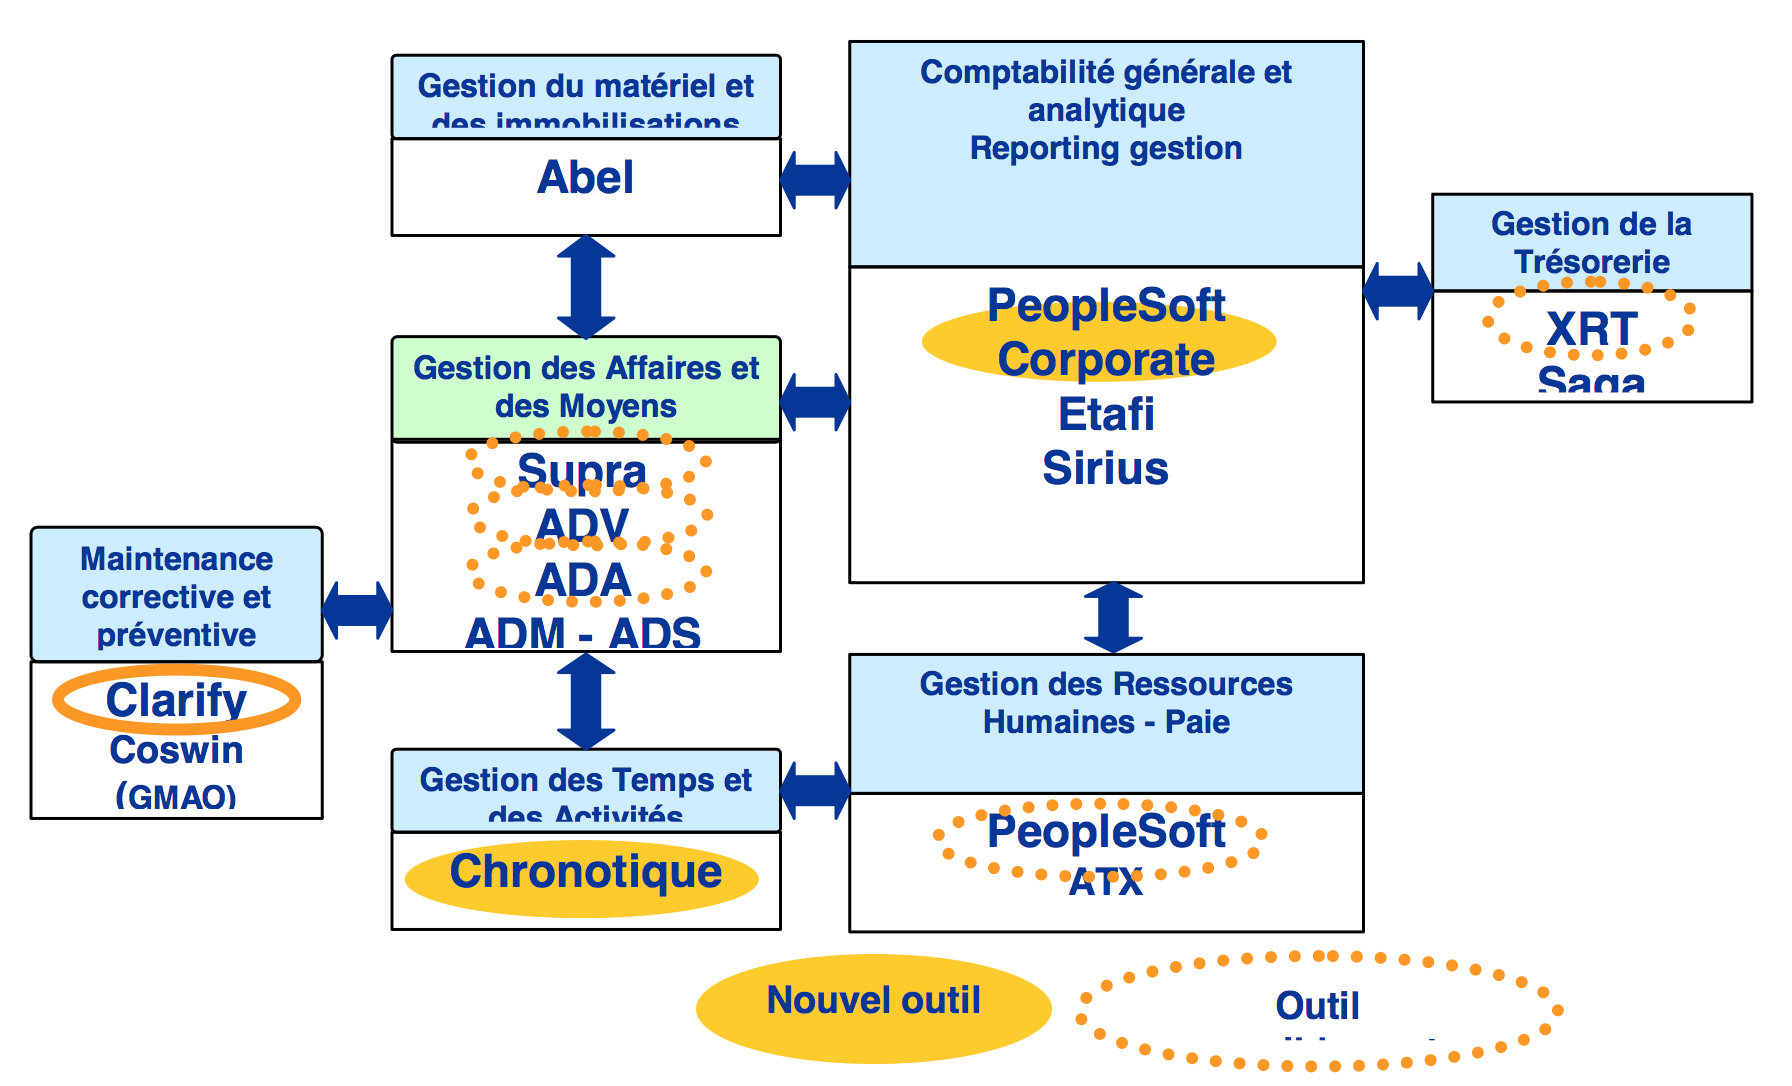
\includegraphics[width=140mm]{A_SI_actuelles.png}
    \caption{Cartographie g\'en\'erale du SI de SPIE}
    \label{diagram:si_map}
\end{figure}

Les attentes du clients sont~:

\begin{itemize}
    \item Pour la solution standard : \'evoluer vers un ERP unique (SAP)
    \item Pour les op\'erations de maintenance, souhait de saisir les \'ev\'enements et les comptes rendus \`a la
    sources (nomadisme)
\end{itemize}

